\documentclass[12pt, a4paper, oneside]{ctexart}
\usepackage{amsmath, amsthm, amssymb, appendix, bm, graphicx, hyperref, mathrsfs,float}
\begin{document}

\title{\textbf{草履虫都能学会的路径积分(量子力学与量子场论,相对论与非相对论,平衡态与非平衡态)}}
\author{拉格朗日的忧郁}
\date{\today}
\linespread{1.5}

\renewcommand{\abstractname}{\Large\textbf{摘要}}


\maketitle

\setcounter{page}{0}
\maketitle
\thispagestyle{empty}

\begin{abstract}
传统量子力学教学往往偏重于正则量子化的讲授,而较少深入讲解路径积分量子化理论。但在现代物理研究中,路径积分已经成为了一套相当主流的语言,因此学会路径积分框架对阅读文献和进行计算都非常重要。本篇笔记主要从最基础的角度对路径积分进行介绍,并在此基础上介绍量子场论,既包含相对论的高能量子场论,也包含非相对论的凝聚态场论,而且我们会对非平衡态场论进行初步介绍。
\end{abstract}

\newpage

\pagenumbering{Roman}
\setcounter{page}{1}
\tableofcontents
\newpage
\setcounter{page}{1}
\pagenumbering{arabic}

\section{引言}
要问路径积分是什么?我想说路径积分是一双慧眼,帮助我们观察和理解这个世界。

自从狄拉克、费曼提出来了路径积分的框架,我们就终于能从复杂繁琐的正则量子化场论计算的地狱中脱离出来,不用再折腾那一大堆不可对易的算符了。在我们传统的初等量子力学课程中,往往不会涉及到路径积分这一美妙的语言,甚至高等量子力学也不一定讲这个。在笔者的学习经历中,第一次上课学路径积分已经是规范场开篇讲泛函场论的时候了。

我先来讲一点小故事调节一下气氛,大家都知道路径积分和费曼的那段往事,从他高中与最小作用量原理结下不解之缘,到他后来以神奇的思路搞出来量子力学的路径积分表述,简直就是一段传奇。不过从历史的脉络上来讲,路径积分的直接起源可以追溯到控制论的提出者维纳(Wiener),他在研究布朗运动的时候首先开始使用类似于路径积分的操作;在维纳的启发下,量子力学真神之一狄拉克在1933年开始做出了量子力学路径积分表述的最基础思路,并指出来了鞍点(saddle point)在联系量子与经典之间的重要性,但狄拉克并没有彻底解决路径求和计算,只是提出来了这么一个思想。在狄拉克思路的影响下,费曼最终在1948年完成了路径积分的开发,而自此开始,我们触摸到了全新的世界。

尽管路径积分听起来相当高大上,但其基本思想和计算确是相当的简单明了,我们只需要很简单的前置知识就能搞明白路径积分量子场论到底是怎么回事,只要没有畏难情绪,我们就可以轻松击破一切障碍。标题说的草履虫肯定只是在吸引大伙的目光,基础还是需要一点点的,但是不会太复杂,只会涉及到一点简单计算而已。先列一下基础知识:
\begin{itemize}
    \item 量子力学需要知道左矢右矢、算符、完备性关系、坐标基矢和动量基矢的转化关系、薛定谔方程、幺正演化算符、二次量子化。
    \item 统计力学需要知道配分函数和密度矩阵。
    \item 经典力学需要知道拉氏量和哈密顿量一般长啥样。(一个$T-V$,一个$T+V$ )。
    \item 数学需要会高斯积分。
\end{itemize}



我写这篇文章的目的有三:一是系统梳理我们所接触到的各种路径积分的框架,不要一叶障目,而是看到各种路径积分的共通性;二是我计划做一些非平衡态的工作,我的套路是在路径积分泛函场论的框架下进行处理,所以也要把非平衡态的东西放进这套框架,但直接写非平衡态路径积分容易把自己和别人都搞糊涂,所以就系统做一个梳理,顺便写一些非平衡态场论的文章和笔记放到知乎上,现在我在试用新的国产latex线上编译平台loongtex,所以顺便利用这个平台把之前的notes整理成latex文档;三是给大伙做个参考,看看路径积分这套玩意儿怎么玩。

现在废话不多说,路径积分,启动!

\section{量子力学中的路径积分}
在量子力学的路径积分计算中,处于最中心地位的问题,对于哈密顿量为$\hat H$的系统,粒子从初态$\left|  q_I \right>$经过时间$t$的演化到末态$\left|  q_F \right>$(假定是粒子从某个位置跑到另一个位置)的振幅是多大,这个振幅一般长这样:
\begin{equation}
    U(q_F,t;q_I,0)=\left< q_F | e^{-i\hat HT} | q_I \right>.
\end{equation}
利用量子力学的基本框架,我们总可以把这个问题清清楚楚明明白白算出来。但路径积分的思路稍有不同,路径积分说白了就是要让我们去看含时演化的具体细节,要让演化一步一步慢慢进行,每演化一步,都要拍个照片,要去看相应所有可能的振幅,然后把这些振幅求和。我们实际操作一下好了,首先拿一把大砍刀把时间均匀切成无数个非常非常小的切片(就像鲁智深让郑屠切肉一样“要十斤精肉,切作臊子”):
\begin{equation}
    e^{-i\hat HT}=\lim_{M\rightarrow\infty}\prod_{l=1}^Me^{-i\hat H\delta t}.
\end{equation}
其中$\delta t=T/M$。然后我们要在两个相邻的$e^{-i\hat H\delta t}$之间插入一个完备基:
\begin{equation}
    \int dq\left| q \right> \left< q \right|=1.
\end{equation}
这样一来,我们就能把每一步演化的振幅轻松拿捏了,直接写出来:
\begin{align} 
\left< q_F | e^{-i\hat HT} | q_I \right>=&(\prod_{l=1}^{M-1}\int dq_l) \left< q_F | e^{-i\hat H\delta t} | q_{M-1} \right>\left< q_{M-1} | e^{-i\hat H\delta t} | q_{M-2} \right>\cdots\nonumber\\ 
&\left< q_{l+1}| e^{-i\hat H\delta t} | q_{l} \right>\cdots \left< q_{1}| e^{-i\hat H\delta t} | q_{I} \right> 
\end{align}
我们现在拿出其中的某一项$\left< q_{l+1}| e^{-i\hat H\delta t} | q_{l} \right>$来观察,这个中间时刻的振幅就反映了量子力学演化的细节。为了搞清楚这一项振幅等于多少,我们考虑最简单的情形,也就是自由粒子的哈密顿量:
\begin{equation}
    \hat H=\hat p^2/(2m)
\end{equation}
假设我们这里取的完备基是坐标表象的基矢$\{ \left| q \right> \}$,注意到此时哈密顿量的本征态和动量本征态是一致的,记为$\left| p \right>$,我们还知道动量本征态在坐标空间就是平面波,即$\left< q | p \right>=e^{ipq}$,动量完备基一般记为$\int dp/(2\pi)\left| p \right>\left< p \right|=1$。利用这里的这些结论,我们马上就能把上面那个矩阵元给解出来:
\begin{align} 
\left< q_{l+1}| e^{-i\hat H\delta t} | q_{l} \right>=&\int \frac{dp}{2\pi}\left< q_{l+1}| e^{-i\hat H\delta t} | p \right>\left< p| q_l \right>\nonumber\\ 
=&\int \frac{dp}{2\pi}\left< q_{l+1}| e^{-i\frac{p^2}{2m}\delta t} | p \right>e^{-ipq_l}\nonumber\\ 
=&\int \frac{dp}{2\pi}e^{-i\frac{p^2}{2m}\delta t}e^{ipq_{l+1}}e^{-ipq_l}\nonumber\\ 
=&\int \frac{dp}{2\pi}e^{-i\frac{p^2}{2m}\delta t}e^{ip(q_{l+1}-q_l)}\nonumber\\ 
=&(\frac{m}{2\pi i\delta t})^{1/2}e^{i\delta t(m/2)[(q_{l+1}-q_l)/\delta t]^2} \label{eq:qmintegral}
\end{align}
这里最后一步用到了高斯积分公式。我们把所有振幅都乘起来,并对所有可能性进行积分,马上就能得到最终的振幅结构:
\begin{align} 
\left< q_F | e^{-i\hat HT} | q_I \right>=&(\frac{m}{2\pi i\delta t})^{M/2}(\prod_{k=1}^{M-1}\int dq_k) e^{i\delta t(m/2)\sum_{l=0}^{M-1}[(q_{l+1}-q_l)/\delta t]^2} 
\end{align}
我们很容易发现原本的哈密顿量被转换成了拉氏量,事实上加入相互作用的结果也是类似的:
\begin{equation}
    \left< q_F | e^{-i\hat HT} | q_I \right>=\int D[q]e^{i\int_0^T dt L(\dot q,q)}
\end{equation}
这个我们一般倾向于通过一个Wick转动$t\rightarrow -i\tau$来把积分转到欧式时空,不过这个其实不重要,因为很多时候我们压根不需要真正把这个积分积出来,而是直接探讨关联函数之间的关系。
还需要说明的一点是,在路径积分的问题中,有一种常见的做法是直接把初末态选为真空态。

\section{多自由度量子力学与相对论性路径积分场论}
要通往量子场论,我们就要去考虑多自由度的路径积分,这个做起来也很简单。我们考虑一个$N$粒子的情形,其哈密顿量为:
\begin{equation}
    H=\sum_a\frac{1}{2m_a}\hat p_a^2+V(\hat q_1,\cdots,\hat q_N)
\end{equation}
利用之前的办法,我们依然在时间演化上插入一大堆完备基,只不过这个时候的完备基是一个多粒子态的完备基,我们直接把结果写出来:
\begin{equation}
    Z\equiv\left< 0 |e^{-iHT}| 0 \right>=\int D[q]e^{iS[q]}
\end{equation}
其中作用量就是对多粒子拉氏量时间的积分:
\begin{equation}
    S[q]=\int_0^T d t (\sum_a\frac{1}{2m_a}\dot q_a^2-V[q_1,q_2,\cdots,q_N])
\end{equation}
接下来我们利用完全相同的思路考虑一般的相对论场论。在量子力学中,坐标是算符而时间是参数,两者完全不是一码事,在量子场论中,我们将同时把坐标和时间作为参数,写出来场算符$\hat\psi(\bm x,t)\equiv \hat\psi(x)$。对比上面的多自由度量子力学,把$a$当作坐标自由度$\mathbf x$,而$q$当作场,对应场$\psi(\bm x,t)$。原本的积分求和将变成:
\begin{equation}
    \int_0^t d t\sum_a\rightarrow \int d^Dx
\end{equation} 
动能项将变成$\int d^D x \frac{1}{2}(\partial\psi/\partial t)^2$。而相互作用一般可以作这样的展开(类似于胡克定律):
\begin{equation}
    V(q_1,\cdots,q_N)=\sum_{ab}\frac{1}{2}k_{ab}(q_a-q_b)^2+\cdots
\end{equation}
我们把这样的相互作用转化到场论中,考虑相邻$a,b$代表的空间位置是$\mathbf x_a,\mathbf x_b$,而$k_{ab}$要求两个空间位置必须相邻,然后我们考虑空间要连续化(让$\mathbf x_a,\mathbf x_b$相距无穷小),于是相互作用项就变成:
\begin{equation}
    \int d^Dx(\partial\psi/\partial \bm x)^2
\end{equation}
最后我们会得到一个洛伦兹不变的量子场论:
\begin{equation}
    Z=\int D[\psi]e^{iS[\psi]},
\end{equation}

\begin{equation}
    S[\psi]=\int d^Dx\mathcal L[\psi(x)].
\end{equation}
而这种标量场拉氏量经常包含下面这些项
\begin{equation}
    \mathcal L=\frac{1}{2}\partial^\mu\psi\partial_\mu\psi-\frac{1}{2}m\psi^2-\frac{\lambda}{4!}\psi^4+\cdots.
\end{equation}
不过最一般的形式一般是:
\begin{equation}
    \mathcal L=\frac{1}{2}\partial^\mu\psi\partial_\mu\psi-V(\psi).
\end{equation}
这里对路径积分泛函场论部分的引入和推导主要强调概念的引入,不注重具体数学的严格处理,所以没有具体解释系数的计算。我们这里还是稍微总结一下,我们得到生成泛函的方式实际上是把演化算符给切成了臊子。

一般的演化算符是$\hat U(t_2,t_1)=\mathcal T e^{-i\int_{t_1}^{t_2}H(t)dt}$,我们取正负无穷远的时间都是基态,于是就得到了生成泛函的表达式:
\begin{equation}
    Z=\left<\Omega |\hat U(+\infty,-\infty)| \Omega \right>.
\end{equation}
其中不断插入完备基就能得到上面的路径积分生成泛函的形式,也就是上面那种结构,感兴趣的小伙伴可以自己试着推一下,也可以翻翻场论书。

\section{哈密顿量形式的路径积分量子力学}
在凝聚态和统计物理中所使用的场论一般是非相对论场论,在这类问题中,我们一般不使用拉氏量,而是用哈密顿量去构造作用量。两者有着微妙的不同,拉氏量的形式很方便用来刻画具有洛伦兹不变性的系统,而在凝聚态问题中,我们往往是哈密顿量起手,所以用哈密顿量去构造作用量反而来得更方便。为了进一步说明这个问题,我们还是以自由粒子的量子力学问题为例进行计算,考虑振幅
\begin{equation}
    \left< q_F | e^{-i\hat HT} | q_I \right>
\end{equation}
同样拆成特别多份,让我们回到上面这一步Eq.~(\ref{eq:qmintegral})的计算中:
\begin{align} 
\left< q_{l+1}| e^{-i\hat H\delta t} | q_{l} \right>=&\int \frac{dp}{2\pi}\left< q_{l+1}| e^{-i\hat H\delta t} | p \right>\left< p| q_l \right>\nonumber\\
 =&\int \frac{dp}{2\pi}\left< q_{l+1}| e^{-i\frac{p^2}{2m}\delta t} | p \right>e^{-ipq_l}\nonumber\\
  =&\int \frac{dp}{2\pi}e^{-i\frac{p^2}{2m}\delta t}e^{ipq_{l+1}}e^{-ipq_l}\nonumber\\ 
  =&\int \frac{dp}{2\pi}e^{-i\frac{p^2}{2m}\delta t}e^{ip(q_{l+1}-q_l)}.
\end{align}
注意这里对动量$p$的积分不要做出来,然后直接把所有时间切片的项都乘起来:
\begin{align}  
\left< q_F | e^{-i\hat HT} | q_I \right>=\lim_{M\rightarrow\infty}&(\prod_{k=1}^{M}\int \frac{dp_k}{(2\pi)^{D-1}}) (\prod_{k=1}^{M-1}\int dq_k) e^{i\sum_{l=0}^{M-1}[p_k(q_k-q_{k-1})-\delta t\frac{p_k^2}{2m}]}  
\end{align}
最后我们做一个连续化,具体来说就是
\begin{equation}
    p_k(q_k-q_{k-1})=p_k\frac{q_k-q_{k-1}}{\delta t} \delta t\rightarrow p_k\dot q_k\delta t.
\end{equation}
于是我们得到了另一种路径积分的形式:
\begin{equation}
    \left< q_F | e^{-i\hat HT} | q_I \right>=\int D[x(t),p(t)]e^{iS},
\end{equation}
\begin{equation}
    S=\int dt (p(t)\dot q(t)-H(p(t),q(t))).
\end{equation}
具体选择什么样的路径积分形式,这取决于我们研究什么问题。在后续的讨论中,我们一般在凝聚态场论中选择这种哈密顿量的形式。

\section{单粒子配分函数遇到路径积分}
我们还得再准备一个小故事,那就是有限温的单粒子量子力学问题,这时我们需要计算的就是配分函数,即
\begin{equation}
    Z=\mathrm{Tr}\{ e^{-\beta H} \}=\int dq \left<q |e^{-\beta H}| q \right>.
\end{equation}
这个地方我们不用去硬算,只需要对比纯态的路径积分和这里有限温的混态路径积分,注意两个基本特征,其一是,此时的初态末态是相同的,都是$\left| q \right>$,这意味着我们只需要对对角元求和;其二是引入虚时$-\beta\rightarrow iT$,这意味着虚时$\tau=-it$。这样一来,我们只需要把纯态量子力学路径积分的结论中的时间换成虚时,然后积分时记得初末态要相等,也要进行积分,就大功告成啦。我们下面具体进行表述:
\begin{align}
    iS=&i\int dt (p(t)\dot q(t)-H(p(t),q(t)))\nonumber\\
    & \Rightarrow\nonumber\\ 
    &-\int_0^\beta d\tau(p(\tau)\dot q(\tau)-H(p(\tau),q(\tau)))
\end{align}
所以我们就直接得到了一个有限温的量子力学路径积分:
\begin{equation}
    Z=\int D[p,q]e^{-S},
\end{equation}
\begin{equation}
    S=\int_0^\beta d\tau(p(\tau)\dot q(\tau)-H(p(\tau),q(\tau))).
\end{equation}
OK,我们接下来用类似的思路来做非相对论的路径积分量子场论。

\section{非相对论性的路径积分量子场论}
\subsection{相干态表象}
要想真正把场论的路径积分给说明白,我们得简单介绍一下相干态表象。首先回忆一下上面的量子力学路径积分我们用过什么表象呢?坐标和动量。为什么要用这样的表象呢?很简单,因为我们用的哈密顿量是$\hat H=\hat p^2/2m+\hat V(r)$,其中包含的关键算符就是动量算符和位置算符,用坐标本征态和动量本征态就是最自然的。那么对于一个多粒子系统,由于微观粒子全同性,我们最好使用二次量子化去表述哈密顿量,换句话说,我们需要用产生湮灭算符(场算符)$\hat a,\hat a^\dagger$去表述哈密顿量。那么很自然地,我们就应该去用产生湮灭算符的本征态去作为完备基来构造路径积分。因此,我们这里要简单介绍一下相干态表象,也就是湮灭算符的本征态。

先针对玻色子的情形进行说明。

首先产生湮灭算符对应的态空间是所谓的Fock空间,在这个空间中我们只去数某个态上的粒子有几个,态矢量一般写成:
\begin{equation}
    \left| n_{\alpha_1},\cdots,n_{\alpha_N}  \right>.
\end{equation}
这里的$1,\cdots,N$标记不同的态,比如在格点系统上,有$N$个格点,第$i$个格点上的有$n_{\alpha_i}$个粒子,就可以用上面的多体Fock态来刻画。
而产生算符就是能让这个态多一个粒子,湮灭算符就是能让这个态少一个粒子:
\begin{align}
    \hat a_{\alpha_i}\left| n_{\alpha_1},n_{\alpha_2},\cdots  \right>&=\sqrt{n_{\alpha_i}} \left| n_{\alpha_1},n_{\alpha_2},\cdots  n_{\alpha_i}-1,\cdots\right>\nonumber\\ 
    \hat a_{\alpha_i}^\dagger\left| n_{\alpha_1},n_{\alpha_2},\cdots  \right>&=\sqrt{n_{\alpha_i}+1} \left| n_{\alpha_1},n_{\alpha_2},\cdots  n_{\alpha_i}+1,\cdots\right>\\
\end{align}
显然这样能告诉我们每个态有几个粒子的Fock态$\left| n_{\alpha_1},\cdots,n_{\alpha_N}  \right>$不可能是产生湮灭算符的本征态,而我们需要的是恰恰就是本征态。所以我们要简单看一下相干态表象怎么得到,首先我们把一个Fock空间的任意波函数用粒子数的基矢做一个展开:
\begin{equation}
    \left|  \phi \right>=\sum_{n_{\alpha_1},n_{\alpha_2},\cdots}\phi_{n_{\alpha_1}n_{\alpha_2}\cdots}\left|  n_{\alpha_1},n_{\alpha_2},\cdots,n_{\alpha_i},\cdots \right>.
\end{equation}
然后我们考虑如果$\left| \phi \right>$如果是湮灭算符的本征态,即相干态
\begin{equation}
    \hat a_{\alpha_i}\left| \phi  \right>=\phi_{\alpha_i}\left| \phi  \right>.
\end{equation}
那么就会得到一个系数条件:
\begin{equation}
    \sqrt{n_{\alpha_1}}\phi_{n_{\alpha_1}n_{\alpha_2}\cdots n_{\alpha_i}\cdots}=\phi_{\alpha_i}\phi_{n_{\alpha_1}n_{\alpha_2}\cdots (n_{\alpha_i}-1)\cdots}.
\end{equation}
我们再做一个归一化的假设,即真空态系数为1,那么我们立刻就能得到相干态的系数表达式:
\begin{equation}
    \phi_{n_{\alpha_1}n_{\alpha_2}\cdots n_{\alpha_i}\cdots}=\frac{\phi_{\alpha_1}^{n_{\alpha_1}}}{\sqrt{n_{\alpha_1}!}}\frac{\phi_{\alpha_2}^{n_{\alpha_2}}}{\sqrt{n_{\alpha_2}!}}\cdots\frac{\phi_{\alpha_i}^{n_{\alpha_i}}}{\sqrt{n_{\alpha_i}!}}\cdots.
\end{equation}
系数有了,我们再对基矢做一点小小的操作,把所有的多粒子态全部变换回真空态,即:
\begin{equation}
    \left|  n_{\alpha_1},n_{\alpha_2},\cdots,n_{\alpha_i},\cdots \right>=\frac{(\hat a^\dagger_{\alpha_1})^{n_{\alpha_1}}}{\sqrt{n_{\alpha_1}!}}\frac{(\hat a^\dagger_{\alpha_2})^{n_{\alpha_2}}}{\sqrt{n_{\alpha_2}!}}\cdots\frac{(\hat a^\dagger_{\alpha_i})^{n_{\alpha_i}}}{\sqrt{n_{\alpha_i}!}}\cdots\left| 0 \right>.
\end{equation}
这样一来我们就能把相干态具体写清楚了:
\begin{equation}
    \left| \phi \right>=\sum_{n_{\alpha_1}\cdots n_{\alpha_i}\cdots}\frac{(\phi_{\alpha_1}\hat a^\dagger_{\alpha_1})^{n_{\alpha_1}}}{{n_{\alpha_1}!}}\frac{(\phi_{\alpha_2}\hat a^\dagger_{\alpha_2})^{n_{\alpha_2}}}{{n_{\alpha_2}!}}\cdots\frac{(\phi_{\alpha_i}\hat a^\dagger_{\alpha_i})^{n_{\alpha_i}}}{{n_{\alpha_i}!}}\cdots\left| 0 \right>.
\end{equation}
如果你还记得高数中最常见的级数展开式,$e^x=\sum_{n=0}^{\infty}x^n/n!$,就立马能意识到上面的这一大坨东西可以直接写成$e$指数的形式:
\begin{equation}
    \left| \phi \right>=e^{\sum_{\alpha}\phi_\alpha \hat a^\dagger_\alpha}\left| 0 \right>.
\end{equation}
当然反过来厄米共轭则是:
\begin{equation}
    \left<\phi \right|=\left< 0 \right|e^{\sum_{\alpha}\phi_\alpha^* \hat a_\alpha}.
\end{equation}
利用这一基本定义我们可以给出如下的性质:
\begin{equation}
    a_{\alpha}^\dagger\left| \phi \right>=a_{\alpha}^\dagger e^{\sum_{\alpha'}\phi_{\alpha'}\hat a^\dagger_{\alpha'}}\left| 0 \right>=\frac{\partial}{\partial\phi_\alpha}\left| \phi \right>.
\end{equation}
\begin{equation}
    \left< \phi \right|\hat a_\alpha=\frac{\partial}{\partial\phi^*_\alpha}\left< \phi \right|.
\end{equation}
\begin{equation}
    \left<\phi |\phi' \right>=e^{\sum_{\alpha}\phi_{\alpha}^*\phi_{\alpha}'}.
\end{equation}
\begin{equation}
    1=\frac{1}{2\pi i}\prod_\alpha d\phi^*_{\alpha}d\phi_{\alpha}e^{-\sum_\alpha \phi^*_{\alpha}\phi_{\alpha}}\left|  \phi_{\alpha} \right> \left<  \phi_{\alpha}\right|.
\end{equation}
\begin{align} 
\mathrm{Tr}\hat A=&\sum_{n}\left<n |\hat A| n\right>\nonumber\\
 =&\sum_n\int \prod_\alpha \frac{1}{2\pi i}d\phi^*_{\alpha}d\phi_{\alpha}e^{-\sum_\alpha \phi^*_{\alpha}\phi_{\alpha}}\left< n |  \phi \right> \left<  \phi\right|\hat A\left| n\right>\nonumber\\ 
 =&\sum_n\int \prod_\alpha \frac{1}{2\pi i}d\phi^*_{\alpha}d\phi_{\alpha}e^{-\sum_\alpha \phi^*_{\alpha}\phi_{\alpha}} \left<  \phi\right|\hat A\left| n\right>\left< n |  \phi \right>\nonumber\\ 
 =&\int \prod_\alpha \frac{1}{2\pi i}d\phi^*_{\alpha}d\phi_{\alpha}e^{-\sum_\alpha \phi^*_{\alpha}\phi_{\alpha}} \left<  \phi|\hat A| \phi \right>.
\end{align}
至于费米子,情况就稍微有所不同了,由于其交换反对称的特点,我们需要用Grassmann数进行刻画。其最基本的性质是:
\begin{equation}
    \xi_\alpha \xi_\beta+\xi_\beta\xi_\alpha=0.
\end{equation}
利用这一特殊的数,我们可以类似地分析费米子的相干态表象,这里限于篇幅就不仔细讨论了,而是直接给出结论。
\begin{figure}[h!]
    \centering
    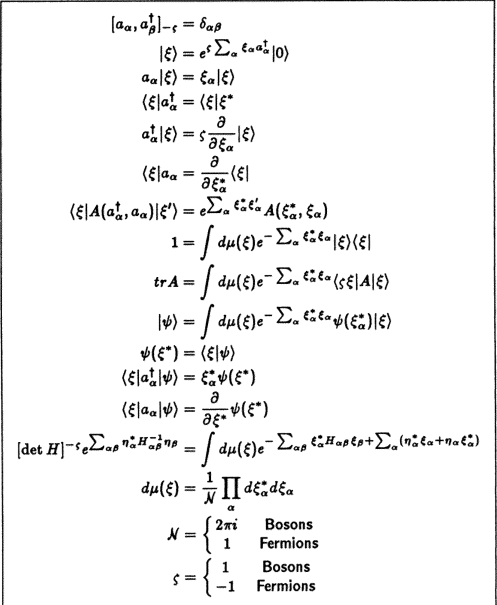
\includegraphics[width=1\textwidth]{coherent_relation.png}
    \caption{相干态表象基本关系\cite{a}}
\end{figure}

总之,我们利用这个表象就可以很快乐地直接拿到场论的路径积分形式了,下面我们就详细说明如何做到这件事情。

\subsection{零温情形}
这一段故事我们要稍微仔细讲一下(上面相对论场论的情形我们是用一个比方一笔带过了,这也是大部分场论书的做法)。利用我们上面讲的相干态表象,我们就能很轻松地把哈密顿量表示出来,不然你随便选一组基,哈密顿量直接变得巨复杂无比,就没意思了。具体的相干态表象的规则在上面列过了,我们这里直接当工具来用就OK,首先给出某个时间切片下的相干态表象的完备性关系:
\begin{equation}
    1=\frac{1}{\mathcal N}\prod_\alpha \int d\phi^*_{\alpha,k}d\phi_{\alpha,k}e^{-\sum_\alpha \phi^*_{\alpha,k}\phi_{\alpha,k}}\left|  \phi_{\alpha,k} \right> \left<  \phi_{\alpha,k}\right|
\end{equation}

这里$\alpha$是标记不同的多体态(例如不同的格点),而$k$则是时间切片的指标。然后我们为方便把哈密顿量按照正规序进行调整,即把所有产生算符扔到左边,把湮灭算符扔到右边,下面出现的哈密顿量默认是正规序的。但等放到指数上面$e^{\delta t \hat H(a^\dagger,a)}$后,即便哈密顿量是正规的,指数展开后也不正规了,不过不用担心,不正规的项的最低阶是在$(\delta t\hat H)^2$,也就是说
\begin{equation}
    e^{\delta t \hat H(a^\dagger,a)}=:e^{\delta t \hat H(a^\dagger,a)}:+\mathcal O(\delta t^2).
\end{equation}
其中$:e^{\delta t \hat H(a^\dagger,a)}:$是指把算符按照正规序进行调整,所以在这个处理中,理论天然会带一个$\mathcal O(\delta t^2)$的系统误差,但这个误差可以通过增大时间切片的数量来进行压低,在无穷多切片的极限误差下可以忽略,因此不用担心这里的误差问题。

然后我们直接算一下振幅,注意,我们这里最好选初末态都是相干态,正如量子力学路径积分时,我们选择初末态是位置本征态一样:
\begin{align} 
U(\phi^*_{\alpha,f},t_f;\phi_{\alpha,i},t_i)=&\left<\phi_f |  e^{-i\int_{t_i}^{t_f}dt \hat H} | \phi_i \right>\nonumber\\ 
=&\lim_{M\rightarrow\infty}\int\prod_{k=1}^{M-1}\prod_{\alpha}d\phi^*_{\alpha,k}d\phi_{\alpha,k}e^{-\sum_{k=1}^{M-1}\sum_\alpha\phi^*_{\alpha,k}\phi_{\alpha,k}}\nonumber\\ 
&\prod_{k=1}^M\left< \phi_k | :e^{-i\delta t \hat H(a^\dagger, a)}:+\mathcal{O}(\delta t^2) |  \phi_{k-1} \right>\nonumber\\ 
=&\lim_{M\rightarrow\infty}\int\prod_{k=1}^{M-1}\prod_{\alpha}d\phi^*_{\alpha,k}d\phi_{\alpha,k}e^{-\sum_{k=1}^{M-1}\sum_\alpha\phi^*_{\alpha,k}\phi_{\alpha,k}}\nonumber\\
 &e^{\sum_{k=1}^M\{ \sum_\alpha \phi^*_{\alpha,k}\phi_{\alpha,k-1} -i\delta t H(\phi^*_{\alpha,k},\phi_{\alpha,k-1})\}}.    
\end{align}
最后一步我们用了相干态的overlap关系$\left<  \phi|\phi' \right>=\exp(\phi^*\phi')$。总之,一旦连续化,我们马上就可以得到
\begin{align} 
U(\phi^*_{\alpha,f},t_f;\phi_{\alpha,i},t_i) =&\int D[\phi^*\phi]e^{\sum_\alpha\phi^*_{\alpha}(t_f)\phi_{\alpha}(t_f)}\nonumber\\ 
&e^{i\int_{t_i}^{t_f} dt\{ \sum_\alpha i \phi^*_{\alpha}(t)\partial_t \phi_\alpha(t)-H(\phi^*,\phi) \}} 
\end{align}
如果去掉末态的常数项,我们就得到了生成泛函和对应的作用量:
\begin{equation}
    Z=\int D[\phi^*\phi]e^{iS}
\end{equation}
\begin{equation}
    S=\int_{t_i}^{t_f}dt [i\phi^*\partial_t\phi-H(\phi^*,\phi)]
\end{equation}
不过注意,如果是严格计算离散时的振幅,那还是把项写全了比较好。总之,这样一来我们就能把零温场论做出来了。

\subsection{有限温情形}
接下来我们再讨论一下有限温的相干态表象路径积分应该怎么做。起手式还是配分函数:
\begin{align}
 Z=&\mathrm{Tr} e^{-\beta(\hat H-\mu\hat N)}\nonumber\\ 
 =&\int \prod_\alpha d\phi^*_\alpha d\phi_\alpha e^{-\sum_{\alpha}\phi^*_\alpha\phi_\alpha}\left<\zeta\phi |e^{-\beta(\hat H-\mu\hat N)}| \phi  \right>  
 \end{align}
这里费米子$\zeta=-1$,玻色子$\zeta=1$,之所以求迹会出现这个结构是来源于相干态表象的基本性质,这里只需要使用这个结论,相干态表象详细推导之后单开一篇。

这里我们只需要类比上面零温的情况,把插入无数的完备性关系,然后把每个平均都给算出来就可以了,这里和上面的振幅没有什么区别。对照刚才的推导,我们可以得到
\begin{equation}
    Z=\lim_{M\rightarrow\infty}\int\prod_{k=1}^M\prod_\alpha\frac{1}{\mathcal N}d\phi_{\alpha,k}^*d\phi_{\alpha,k}e^{-S[\phi^*,\phi]}
\end{equation}
\begin{align}
    S[\phi^*,\phi]=&\delta \tau\sum_{k=2}^M[\sum_\alpha \phi_{\alpha,k}^*\{  \frac{\phi_{\alpha,k}-\phi_{\alpha,k-1}}{\delta \tau} -\mu\phi_{\alpha,k-1} \}+H(\phi^*_{\alpha,k},\phi_{\alpha,k-1})]\nonumber\\ 
    &+\delta\tau[\sum_\alpha \phi^*_{\alpha,1}\{  \frac{\phi_{\alpha,1}-\zeta\phi_{\alpha,kM}}{\delta \tau} -\mu\zeta\phi_{\alpha,M} \}  +H(\phi^*_{\alpha,1},\zeta\phi_{\alpha,M})]\label{eq:dis-action}.
\end{align}
在连续极限下,我们可以写出来一个更常见的配分函数/生成泛函:
\begin{equation}
    Z=\int_{\phi_\alpha(\beta)=\zeta\phi_\alpha(0)} D[\phi^*,\phi]e^{-S[\phi^*,\phi]}.
\end{equation}
\begin{equation}
    S[\phi^*,\phi]=\int_0^\beta d\tau\{ \sum_\alpha \phi^*_\alpha(\tau)(\partial_\tau-\mu)\phi_\alpha(\tau)+H(\phi^*_\alpha,\phi_\alpha)  \}.
\end{equation}
写了一大堆东西,还是太过于抽象了,我们来计算一个具体的模型吧,就拿最简单的自由谐振子系统来举个例子吧,哈密顿是:
\begin{equation}
    \hat H_0=\sum_\alpha \varepsilon_\alpha \hat a^\dagger_\alpha \hat a_\alpha.
\end{equation}
这个哈密顿量天然就是正规序的,也就是产生算符在左边,湮灭算符在右边,就不用我们手动调节了。那配分函数我们把上面式子Eq.~(\ref{eq:dis-action})抄下来就行了:
\begin{align}
    S[\phi^*,\phi]=&\delta \tau\sum_{k=2}^M[\sum_\alpha \phi_{\alpha,k}^*\{  \frac{\phi_{\alpha,k}-\phi_{\alpha,k-1}}{\delta \tau} -\mu\phi_{\alpha,k-1} \}+\varepsilon_\alpha \phi^*_{\alpha,k}\phi_{\alpha,k-1}]\nonumber\\ 
    &+\delta\tau[\sum_\alpha \phi^*_{\alpha,1}\{  \frac{\phi_{\alpha,1}-\zeta\phi_{\alpha,kM}}{\delta \tau} -\mu\zeta\phi_{\alpha,M} \}  +\zeta\varepsilon_k\phi^*_{\alpha,1}\phi_{\alpha,M}]
\end{align}
或者我们写紧凑一点:
\begin{align} 
Z_0=\lim_{M\rightarrow \infty}\prod_\alpha[\prod_{k=1}^n \int \frac{1}{\mathcal N}d\phi_k^*d\phi_k e^{-\sum_{j,k=1}^M \phi_j^* S^{(\alpha)}_{jk}\phi_k}]. 
\end{align}
那么显然$S^{(\alpha)}_{jk}$是个关于虚时指标的矩阵,我们可以直接把这个矩阵给一项一项写出来:
\begin{equation}
    S^{\alpha}= \begin{bmatrix} 1 & 0 &0 & \cdots &0 & -\zeta a\\ -a & 1 &0 &\ddots & &0 \\ 0 & -a & 1 & \ddots & 0 & 0\\ \vdots & 0 &\ddots & & 1& 0\\ 0 & & & \cdots & -a & 1  \end{bmatrix}.
\end{equation}
其中$a=1-\delta t(\varepsilon_k-\mu)=1-\frac{\beta}{M}(\varepsilon_k-\mu)$。

由于自由场时$e$指数上是二次型,也就是说这是个高斯型函数,所以对场的积分可以直接积出来:
\begin{equation}
    Z_0=\lim_{M\rightarrow \infty}\prod_\alpha[\det S^{(\alpha)}]^{-\zeta}.
\end{equation}
我们来把这个行列式算出来,这个行列式的计算实际上是相当简单的,因为每行每列都只有2个位置不为0,你可以直接利用行列式降维来逐阶计算,或者直接查行列式计算公式,或者让mathematica帮你做计算,总之可以得到:
\begin{align} 
\lim_{M\rightarrow\infty}\det S^{(\alpha)}=&\lim_{M\rightarrow\infty}[1+(-1)^{M-1}\zeta(-a)^M]\nonumber\\ 
=&\lim_{M\rightarrow\infty}[1-\zeta(1-\frac{\beta}{M}(\varepsilon_k-\mu))^M]\nonumber\\ 
=&1-\xi e^{-\beta(\varepsilon_k-\mu)}.  
\end{align}
那么自由场的配分函数就能算出来:
\begin{equation}
    Z_0=\prod_\alpha(1-\xi e^{-\beta(\varepsilon_k-\mu)})^{-\zeta}.
\end{equation}
OK,我们拿到了一个特别具体实在的配分函数,这样计算总归是落在了实处上。但是光有配分函数怎么能满足我们的雄心壮志呢?谁家好人能测量配分函数,正经实验学家测的可都是关联函数,所以我们下一小节介绍关联函数的计算。

\section{关联函数}
关联函数到底是啥呢?其实说穿了就是一堆场算符的平均,而平均根据算符在时间上的排列顺序可以分出来很多不同的种类,比如什么retarded、advanced,在其中最特别最特别的是时序关联(time order),即把时间上靠后的算符放到左边,我们具体写一下效果长啥样,比如对下面的时序算符$T$:
\begin{equation}
    T\left\{  \hat O_m(t_m) \hat O_{m-1}(t_{m-1})\cdots \hat O_1(t_1) \right\}.
\end{equation}
如果我们发现$t_m>t_{m-1}>\cdots>t_1$那么时序算符的效果就是:
\begin{equation}
    T\left\{  \hat O_m(t_m) \hat O_{m-1}(t_{m-1})\cdots \hat O_1(t_1) \right\}=\hat O_m(t_m) \hat O_{m-1}(t_{m-1})\cdots \hat O_1(t_1) .
\end{equation}
那如果反过来,让$t_1>t_2>\cdots >t_m$,那么时序算符的效果就是:
\begin{equation}
    T\left\{  \hat O_m(t_m) \hat O_{m-1}(t_{m-1})\cdots \hat O_1(t_1) \right\}=\zeta\hat O_1(t_1) \hat O_{2}(t_{2})\cdots \hat O_m(t_m) .
\end{equation}
($\zeta$是交换可能产生的正负号。)总之时序算符就是这么个意思,对于算符表述来说,时序算符其实相当恶心,这玩意根据算符数目的增多,里面的时间不同排列实在太多了,看着就烦。所以,来,让我们看一下伟大的路径积分下时序关联会变成啥样。

我们就考虑一个最简单的情况,回到量子力学的路径积分下,暂时先忘掉场算符什么什么的,就考虑有俩算符$\hat O_1(\hat q,t_1),\hat O_2(\hat q,t_2)$,然后假设$t_1>t_2$。我们把关联函数写出来:
\begin{equation}
    \left< T\hat O_1(t_1)\hat O_2(t_2)) \right>=\left<q_f|T\hat O_1(\hat q,t_1)\hat O_2(\hat q,t_2)e^{-i\int_{t_i}^{t_f}\hat H(t)dt}| q_i   \right>.
\end{equation}

这个东西应该等于什么呢? 很自然地,你会想到我这个$e$指数上的时间,有时候是大于$t_1$的,有时候是在$t_2$和$t_1$之间的,还有时候是小于$t_2$的,那按照时序算符的定义,是不是就得把$3$指数上的积分拆成三段,按照时间顺序做个简单排列。来,我们把做个想法写成表达式:
\begin{align}
\left< T\hat O_1(t_1)\hat O_2(t_2)) \right>=&\left<q_f | Te^{-i\int_{t_1}^{t_f}\hat H(t)dt}\hat O(\hat q,t_1)  Te^{-i\int_{t_2}^{t_1}\hat H(t)dt} \hat O(\hat q,t_2) Te^{-i\int_{t_i}^{t_2}\hat H(t)dt} | q_i \right>\nonumber\\ 
=&\lim\int \prod_{k=1}^{M-1}dx_k\left<q_f | e^{-i\delta t H}\cdots|q_m \right> \left<q_m | \hat O_1(\hat q)e^{-i\delta t H}|q_{m-1} \right>\cdots\nonumber\\
 =&\int D[q(t)] O_1(q(t_1))O_2(q(t_2))e^{iS}  . 
 \end{align}
类似地,如果你假设$t_2>t_1$,会发现有完全一样的结果。事实上,这就是路径积分表达时序关联的牛逼之处,一旦用路径积分表达,时序关联就会直接被隐藏在路径积分的被积函数里面,完全不用管哪个时间靠前哪个时间靠后。

好啦,记住这个量子力学里面算出来的结论,我们不加证明地直接推广到场论的计算中(想证明也简单,思路都是一样的),定义有限温场论里面的关联函数
\begin{equation}
    G^{(n)}(\alpha_1\tau_1,\cdots \alpha_n\tau_n)=\frac{1}{Z}\int D[\phi]\phi_1(\alpha_1\tau_1)\cdots\phi_n(\alpha_n\tau_n)e^{-S}.
\end{equation}

零温场论和相对论场论也是类似的,只是把$e^{-S}$改成$e^{iS}$而已,再在定义里面加一些虚数单位$i$就行了。另外说明一下这里$\phi_1\cdots\phi_n$可以是$\phi^*$也可以是$\phi$。

那么我们应该怎么从配分函数出发拿到这么一个关联函数呢?很简单,你只需要在作用量中耦合一个外源:
\begin{equation}
    S[\phi;J]=S[\phi]-\sum_\alpha\int d\tau J_{\alpha\tau}\phi_{\alpha}(\tau)-\sum_\alpha\int d\tau J^*_{\alpha\tau}\phi^*_{\alpha}(\tau).
\end{equation}
你只需要对外源求泛函导数,立刻就能得到想要的关联。

举个最简单的例子,单体格林函数:
\begin{equation}
    G(\alpha\tau_1,\gamma\tau_2)=\left< T\hat a_\alpha(\tau_1)\hat a^\dagger(\tau_2) \right>.
\end{equation}
单体格林函数是最简单的关联函数,也是场论中最核心的关联函数,它的重要性怎么说呢,就和星核之于星、星琼之于开拓者一样重要。一切更高阶的关联函数计算都要建立在单体格林函数的基础之上,不算这个压根不行。即便你只有这个单体格林函数,其实你也能搞出来一大堆有意思的玩意儿,比如谱呀、色散呀、费米面呀、能量呀,实在太多了,就不一个一个数了。

啰里八嗦说了一大堆单体格林函数的重要性,主要是想说我们下面算的不是没用的东西,是很重要滴。根据我们前面的分析,Time order的格林函数在路径积分的表达中就是直接把要算的关联算符扔到被积函数中就万事大吉了,我们写出来:
\begin{align}
    G(\alpha_1\tau_1,\alpha_2\tau_2)=&\frac{1}{Z}\int D[\phi^*\phi]\phi_{\alpha_1}(\tau_1) \phi^*_{\alpha_2} (\tau_2)e^{-S[\phi^*,\phi;J,J^*]}\nonumber\\ 
    =&\frac{1}{Z}\int D[\phi^*\phi]\frac{\delta^2}{\delta J^*_{\alpha_2}(\tau_2)\delta J_{\alpha_1}(\tau_1)}e^{-S[\phi^*,\phi;J,J^*]}.
\end{align}
那么还记得我们前面针对自由哈密顿量算出来了配分函数吗?我们可以用类似的办法把自由格林函数给搞出来,还是照旧把离散形式给写出来,引入记号:
\begin{equation}
    \tau_{1} = m_1\frac{\beta}{M} , \quad \tau_{r} = m_2 \frac{\beta}{M}.
\end{equation}
然后我们根据上面的结果去算这个格林函数:

\begin{align} 
G(\alpha_1\tau_1,\alpha_2\tau_2)=  &\frac{1}{Z_{0}}\int \left(\prod_{\delta} \prod_{k = 1}^{M}  \frac{d \phi_{\delta,k}^{\ast} d\phi_{\delta, k}}{\mathcal{N}}\right) e^{-\sum_{i,j = 1}^{M} \phi_{\delta,j}^{\ast} S^{(\delta)}_{jk}\phi_{\delta,k}} \phi_{\alpha, m_1} \phi_{\gamma, m_2}^{\ast} \nonumber\\ 
=&\left.\delta_{\alpha\gamma} \frac{\zeta\partial^{2}}{\partial J_{m_1}^{\ast} \partial J_{m_2}} \frac{\int \left(\prod_{k} d \phi_{k}^{\ast} d\phi_{k}\right) e^{-\sum_{j,k}\phi_{j}^{\ast} S_{jk}^{(\alpha)}\phi_{k} + \sum_{i}(J^{\ast}_{i}\phi_{i} + \phi_{i}^{\ast}J_{i})}} {\int \left(\prod_{k} d \phi_{k}^{\ast} d\phi_{k}\right)e^{-\sum_{j,k}\phi_{j}^{\ast} S_{jk}^{(\alpha)}\phi_{k}} } \right|_{J=J^{\ast} = 0} \nonumber\\ 
=& \left.\delta_{\alpha\gamma} \frac{\zeta\partial^{2}}{\partial J_{m_1}^{\ast} \partial J_{m_2}} e^{\sum_{j,k}J^{\ast}_{j}S^{(\alpha) ^{-1}}_{jk}J_{k}}\right|_{J=J^{\ast} = 0} \nonumber\\
 =& \delta_{\alpha\gamma}S^{(\alpha) ^{-1}}_{m_1m_2} 
\end{align}
把每一项写出来可以发现
\begin{equation}
    S^{(\alpha)^{-1}} = \frac{1}{1 - \zeta a^{M}} \begin{bmatrix} 1                 & \zeta a^{M - 1} & \zeta a^{M - 2} & \cdots  & \zeta a \\ a                 & 1                            & \zeta a^{M - 1} &  \cdots & \zeta a^{2} \\ a^2            & a                            & 1                            &                & \zeta a^{3} \\ \vdots      &                                &                               & \ddots  &  \vdots \\ a^{M - 1} & a^{M - 2}              & a^{M - 1}            & \cdots  & 1 \end{bmatrix}
\end{equation}
我们对时间顺序做一点分类,然后连续化,就能得到:
\begin{equation}
\lim_{M \rightarrow \infty}S^{(\alpha)^{-1}}_{m_1m_2}  = \left\{\begin{aligned} &e^{-(\epsilon_{\alpha} - \mu) (\tau_{1} - \tau{2})} \left(1 + \zeta n_{\alpha} \right) &\tau_{1} \ge \tau_{2}\\ &e^{-(\epsilon_{\alpha} - \mu)(\tau_{1} - \tau_{2})} \zeta n{\alpha}  & \tau_{1} <  \tau_{2} \end{aligned} \right.
\end{equation}
其中$n_\alpha=\frac{1}{e^{\beta(\varepsilon_k-\mu)}-\zeta}$是玻色/费米分布,这也就是自由格林函数的结果。注意如果$\tau_2=\tau_1-0^+$,即两个场算符的时间几乎相等,湮灭算符时间上稍微靠后一点点,这样我们就计算等时关联$\left< \hat a_\alpha \hat a_\alpha^\dagger \right>=1+\zeta\left<  \hat a_\alpha^\dagger\hat a_\alpha \right>$,把上面格林函数结果带进来,立刻就能发现$\left<  \hat a_\alpha^\dagger\hat a_\alpha \right>=n_\alpha$恰好就等于密度,结果非常物理,完美。

那么关联函数暂且就先告一段落,最基本的已经讲完了,更加技术性的就不在这个简单基础的文章中提及了。

\section{Keldysh场论的路径积分形式}
路径积分这套框架的关键在于要把理论写到具体的表象下面,实现算符到数的转变。我们可以考虑在无穷远过去的场算符$\hat\varphi(\bm x,t=-\infty)$的本征态$\left|  \varphi'(\bm x) \right>$(实际不一定需要,关键是要把你想考虑的演化时间放进来),此时密度矩阵可以展开为:
\begin{equation}
    \hat\rho=\int d\varphi'(\bm x)d\varphi''(\bm x)\left|  \varphi'(\bm x) \right>\rho_{\varphi'\varphi''}\left< \varphi''(\bm x)  \right|.
\end{equation}
于是我们可以把生成泛函展开为:
\begin{equation}
    Z[J]=\int d\varphi'(\bm x)d\varphi''(\bm x)\rho_{\varphi'\varphi''}\left< \varphi''(\bm x)  \right| U(t_-=-\infty,t_+=-\infty)\left|  \varphi'(\bm x) \right>.
\end{equation}
其中$U$是定义在contour上的演化算符,在量子场论框架中,如何把这套东西写成路径积分呢?很简单,直接照抄前面的就行,我们把某一段演化振幅写出来:
\begin{align}
    &\left< \varphi_2(\bm x) |U(t_2,t_1)| \varphi_1(\bm x) \right>\nonumber\\ 
    &=N\int D[\varphi]\exp\{ i\int_{t_1}^{t_2}d^Dx\mathcal{L}[\varphi]  \}\delta(\varphi(\bm x,t_2)-\varphi_2(\bm x))\delta(\varphi(\bm x,t_1)-\varphi_1(\bm x))
\end{align}
这套做法在contour上也同样适用(Keldysh Contour如图\ref{Keldysh}),用完全的办法,我们可以得到Keldysh框架下的路径积分表述:
\begin{align}
    Z[J]=&\int D[\varphi]\exp\{ i\int_pd^Dx(\mathcal{L}[\varphi] -J(x)\varphi(x)) \}\nonumber\\
    &\rho_{\varphi'\varphi''}\delta(\varphi(\bm x,t_+=-\infty)-\varphi'(\bm x))\delta(\varphi(\bm x,t_-=-\infty)-\varphi''(\bm x))
\end{align}
\begin{figure}[h!]
    \centering
    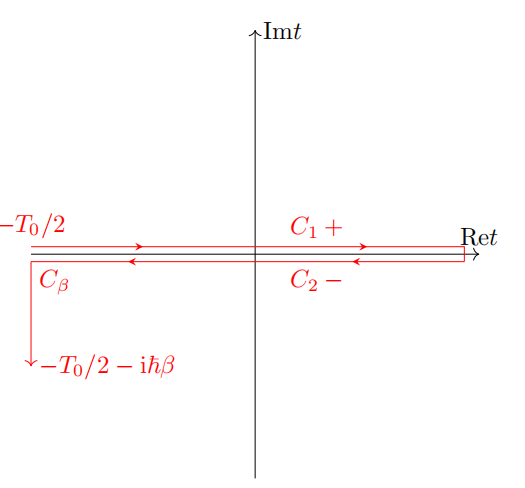
\includegraphics[width=1\textwidth]{Keldysh_contour.png}
    \caption{Keldysh路径\cite{e}}\label{Keldysh}
\end{figure}

至于其余配分函数、格林函数的具体求解,我们在此处就不进行展示了。

\section{小结}
我们这篇小短文简单把路径积分最核心的内容串了一遍,以量子力学为起点开始,然后自然进入量子场论的路径积分表述,不论是相对论的还是非相对论的,是零温还是有限温,是平衡态还是非平衡态,全部给捋下来了,姑且算得上是一场极其有趣的智力冒险。
标题说是草履虫都能懂,主要是把大伙先骗进来,而且我也勉强可以狡辩这里的草履虫指的是琪亚娜·卡斯兰娜。为了尽可能让大家方便理解,我尽量避免太过严重的跳步,并加上了尽可能多的说明和前后文的对比。如果已经看到最后了,想必诸位应该还算有所收获,也希望读者能从中感受到路径积分到底是何等简洁美妙的一套语言,虽然我不信上帝,但我姑且还是想说路径积分是上帝赐给我们的最美妙的礼物。当然不管大伙收获怎么样,我自个儿把这些玩意儿从头整理了一番还是对路径积分有了新的体会和感触。
我希望本文可以作为一个起点,帮助更多人了解路径积分到底是个什么玩意儿,让更多人把路径积分用起来。事实上,在具体研究中,路径积分的量子场论相比传统的正则量子化有非常显著的优势。对于凝聚态问题来说,如果采用路径积分,遇到一个模型,我们不管三七二十一,先把对应的路径积分表示下的生成泛函写出来,然后该加外源加外源,该算关联算关联,像轰炸机一样解决我们遇到的一切问题,这种暴力美学就是我无比钟爱路径积分的原因。

\newpage

\section*{Acknowledgements}
本篇文章的latex框架参考了知乎大佬@Dylaaan编写的latex中文模板,在此特别感谢。同时感谢LoongTex开发团队告诉我还有这么好玩的国产latex线上平台,如果不是恰好被推荐了新平台,可能我就懒得把这篇文章整理成latex文档了。
\newpage

\begin{thebibliography}{99}
    \bibitem{a}Negele J W. Quantum many-particle systems[M]. CRC Press, 2018.
    \bibitem{b}Altland A, Simons B D. Condensed matter field theory[M]. Cambridge University Press, 2010.
    \bibitem{c}Zee A. Quantum field theory in a nutshell[M]. Princeton University Press, 2010.
    \bibitem{d}Chou K, Su Z, Hao B, et al. Equilibrium and nonequilibrium formalisms made unified[J]. Physics Reports, 1985, 118(1-2): 1-131.
    \bibitem{e}北京大学量子材料中心施均仁老师课堂讲义
\end{thebibliography}

\newpage

\end{document}
